\chapter{Theory}\label{chap:theory}

% TODO: Add \refs to sections for (1) and (2) parts of sentence.
This chapter will iterate the theoretical background necessary for understanding how we trap and cool our ions, and the available measures we performed on the simulation results. With respect to trapping, we present 2 small innovations in the field, which are (1) inverse solution of the Mathieu equation, and (2) non-trivial dependence of mass to secular frequencies, which is particularly relevant for thermodynamically stable initial conditions.

\section{Trapping}\label{sec:theory/trapping}

% TODO: Cite more places that solve the Mathieu equation from a geometry of electrodes.
Real-life ion traps are implemented using electrodes designed in a specific geometry, attached to oscillating electric potentials of specific forms. In literature, one often finds attempts to derive analytical expressions for electric potential given a certain geometry and voltages. Usually\cite{AkermanThesis} these derivations are at least somewhat inaccurate, due to the finite size of the electrodes.

LAMMPS is not capable of solving the Laplace equation (\ref{eq:laplace-original}) given a design of electrodes and voltages. Plus, even software tools that do specialize in such calculations (e.g \cite{FEniCS} \& \cite{SIMION}), are not capable of combining also Coulomb interactions\footnote{Developing a software that computes both the Laplace equation \emph{and} Coulomb interactions should be immensely complicated, due to image charges, and I'm unaware of any software tool capable of that.}. Therefor we chose to focus the effort on producing analytical expressions with abstract parameters, that trap our ions in desired secular frequencies. The basic form of the electric field we simulated is:

\begin{equation}
	E_i = (a_i + q_i \cos(\omega_\mathrm{rf} t)) x_i
	\label{eq:mathieu-source}
\end{equation}

For the $i$th spatial dimension, and the dimensions of $a_i$ \& $q_i$ are naturally $\mathrm{Volt}/\mathrm{distance^2}$. The 1D equation of motion you get for a single ion under this field is:

\begin{equation}
	(a + 2 q \cos(2 \tau)) x = \ddot{x}
\end{equation}

% TODO: Cite literature?
Where $2\tau \equiv \omega_\mathrm{rf} t$, and $(a_i, q_i)$ were rescaled to be dimensionless and therefor given no $i$ subscript to reflect that. This is called the Mathieu equation\cite{MathieuOriginal}, and for the sake of completeness, I'll present here how I solved it, in a way that is more tailored for semi-numerical calculations.

\subsection{Solving the Mathieu Equation in 1D}

Substituting the following expression as a solution:

\begin{equation}
x(\tau) = e^{i\beta\tau}\sum_{n=-\infty}^\infty \gamma_n e^{i n \tau} + e^{-i\beta\tau}\sum_{n=-\infty}^\infty \gamma_n e^{-i n \tau}
\end{equation}

Yields the infinite set of equations:

\begin{equation}
	\gamma_{n+1} + \gamma_{n-1} = \frac{\tilde{a}_i - \left(\beta_i + n\right)^2}{\tilde{q}_i} \gamma_n,\quad \forall i\in\{x,y,z\},\ \forall n\in\mathcal{Z}
	\label{eq:gamma_n-relation}
\end{equation}

Where $n\in(-\infty, \infty)$ and $\beta = 2 \omega_\mathrm{sec}/\omega_\mathrm{rf}$. The main point important to understand, is that we need to find a non-trivial solution, meaning a set $\gamma_n$ coefficients that not all are $0$. The best way to view the equations of all coefficients is via a matrix:

\begin{equation}
% Generated by ChatGPT using the Python code :)
\begin{bmatrix}
\ddots & \ddots & \ddots & & & & \vdots & \vdots & \\
\ddots & -D_{-N} & 1 & 0 & \cdots & 0 & 0 & 0 & \cdots \\
\ddots & 1 & \cdots & \cdots & \cdots & \cdots & \cdots & 0 & \cdots \\
& 0 & \cdots & -D_{-1} & 1 & 0 & \cdots & 0 & \\
& \vdots & \cdots & 1 & -D_0 & 1 & \cdots & \vdots & \\
& 0 & \cdots & 0 & 1 & -D_{1} & \cdots & 0 & \\
\cdots & 0 & \cdots & \cdots & \cdots & \cdots & \cdots & 1 & \ddots \\
\cdots & 0 & 0 & \cdots & 0 & 1 & -D_{N} & \ddots & \ddots \\
& \vdots & \vdots & & & \ddots & \ddots & \ddots & \ddots \\
\end{bmatrix}
\begin{bmatrix}
\vdots \\
\gamma_{-N} \\
\vdots \\
\gamma_{-1} \\
\gamma_0 \\
\gamma_{1} \\
\vdots \\
\gamma_{N} \\
\vdots
\end{bmatrix}
\overset{!}{=}
\begin{bmatrix}
\vdots \\
0 \\
\vdots \\
0 \\
0 \\
0 \\
\vdots \\
0 \\
\vdots
\end{bmatrix}
\end{equation}

Where similarly to \ref{eq:gamma_n-relation}:

$$D_n = \frac{a - \left(\beta + n\right)^2}{q}$$

One can easily see that $D_n$ increases $\sim n^2$, which promises the target $\beta$ solution might converge if a finite matrix will be used. To require a non-trivial solution, we simply require the matrix to have a $0$ determinant, thus supplying us an equation for $\beta$ that can be solved easily numerically, for matrix size $2N+1$. Inserting the $\beta$ into the matrix, and inspecting the kernel of it, will give us the $\gamma_n$ coefficients of the solution, and we'd be able to easily verify they indeed decrease with $|n|$, and are that $\gamma_0$ is the most dominant.

The verification of this solution was implemented in a Matplotlib\cite{Matplotlib} based interactive plot, presented in figures \ref{fig:pure-mathieu-coefficients} \& \ref{fig:pure-mathieu-fft}.

\begin{figure}
	\begin{center}
		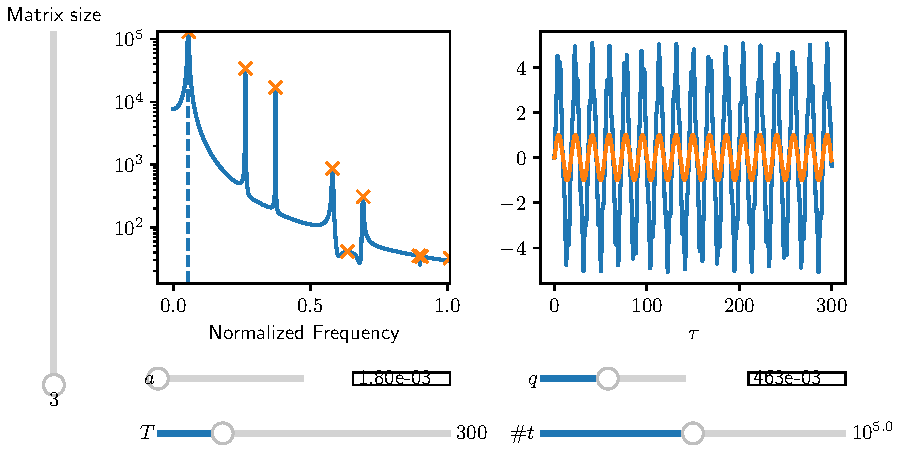
\includegraphics[width=\textwidth]{graphics/pure-mathieu-fft.pdf}
	\end{center}
	\caption{Matplotlib interactive plot presenting the 1 dimensional solution of the Mathieu equation, with a spectrum analysis demonstrating the correct matrix based solution of $\beta$ in the dashed line. The orange sinusoidal line in the right axes is a simple cosine line with the right phase and the calculated $\beta$ as a frequency. The $T$ and $\#t$ sliders control the total time duration of the numerical ODE solution and the amount of time points, respectively.}
	\label{fig:pure-mathieu-fft}
\end{figure}

\begin{figure}
	\begin{center}
		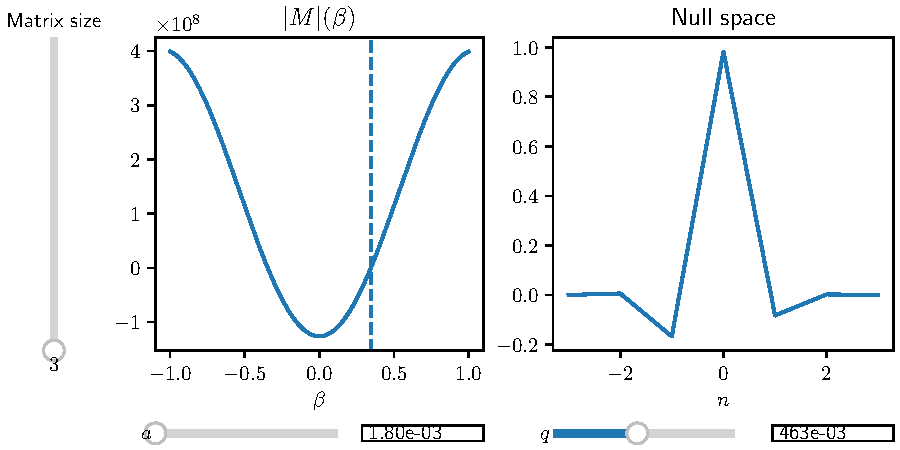
\includegraphics[width=\textwidth]{graphics/pure-mathieu-kernel.pdf}
	\end{center}
	\caption{Matplotlib interactive plot demonstrating the fast decay of the Mathieu equation's solution's $\gamma_n$ (normalized) coefficients, as $|n|$ increases. The dashed $\beta$ line represents the $\beta$ which zeros the matrix determinant.}
	\label{fig:pure-mathieu-coefficients}
\end{figure}

Interactive plot \ref{fig:pure-mathieu-fft} can be also useful for inspecting the roughness of the motion as a function of $a$ and $q$. As expected, a high $q$ and a lower $a$ produce more 'RF-noisy' motion near the peaks of the oscillatory, secular motion. Also, satisfyingly, there's barely any difference in the $\beta$ accuracy as $N$ is increased, even when starting from $N=3$. Hence, this parameter was practically hard-coded in all the simulations etc. to $N=7$.

\subsection{Solving Mathieu Equation Inversely}\label{sec:theory/mathieu-inversly}

Now that we know how to solve the Mathieu equation given $(a_i, q_i)$, and get a secular frequency $\beta_i$, we wish to be able to find a set of 3 $(a_i, q_i)$ pairs per spatial dimension, that will produce a requested set of secular frequencies. The $(a_i, q_i)$ must satisfy the Laplace equation, meaning:

\begin{equation}
	\sum_{i\in{x,y,z}} a_i = \sum_{i\in{x,y,z}} q_i = 0
	\label{eq:laplace}
\end{equation}

So we have now 5 equations, and 6 unknowns. The last equation required to determine a single possible solution, can be:

\begin{equation}
	q_z = 0
\end{equation}

Which is a fair assumption, based on the geometry of our trap, and the typical voltages we put on our electrodes\cite{ElianaThesis}. The best way I found to present the solution to this system of equations, is via a Mathieu stability diagram.

% TODO: Cite this
Most Mathieu stability diagrams found in literature, assume that geometry dictates $a_x = a_y$, and like us, that $q_z = 0$. Thanks to equation \ref{eq:laplace}, this suggests that one can plot a single Mathieu stability diagram for a 3 dimensional trap using a single Mathieu stability diagram for $(a_r,q_r)$ where $a_r \equiv a_x = a_y = -a_z/2$ and $q_r = q_x = -q_y$ as axes. I find these stability diagrams confusing, as they need to also take care of correctly mirroring $q_x = -q_y$ to satisfy stability in both $x$ \& $y$ spatial dimensions (where the $z$ axis is trivially stable). Figure~\ref{fig:mathieu-stability} presents a much simpler approach to show the stability of a 3 dimensional trap, without even imposing cylindrical symmetry which shouldn't be physically impossible.

\begin{figure}
	\begin{center}
		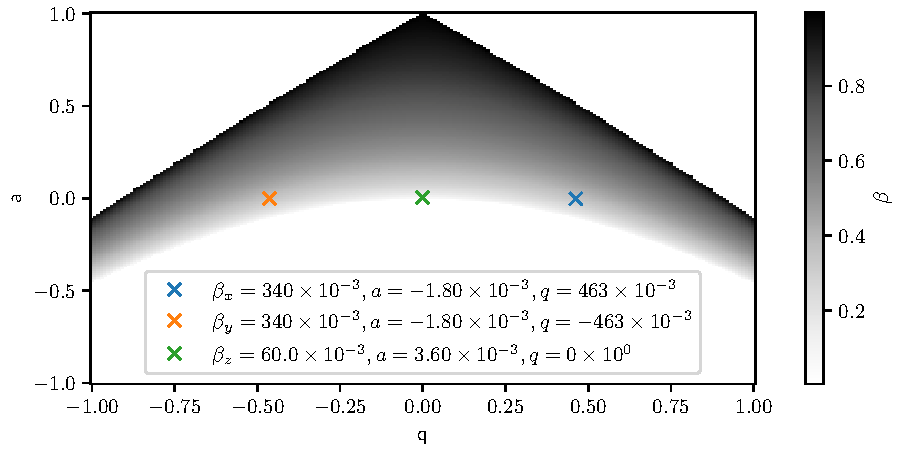
\includegraphics[width=\textwidth]{graphics/pure-mathieu-stability.pdf}
	\end{center}
	\caption{Mathieu Stability diagram, with shades of gray marking the magnitude of $\beta$. The $\times$ signs are specific $\beta$ values, that were used in many simulations of this work - $\beta$s corresponding to secular frequencies $(8.5, 8.5, 1.5)\mathrm{kHz}$, with $f_\mathrm{rf} = 50\mathrm{kHz}$.}
	\label{fig:mathieu-stability}
\end{figure}

\subsection{Initial Conditions \& Coulomb Energy}\label{sec:theory/init-coulomb}

We wish to study sympathetic cooling starting from a thermodynamically stable state. This raises a few important questions: How significant is the Coulomb potential energy in the Boltzmann ensemble? Should it be considered when initiating the positions and velocities of the ions?

Under the secular approximation, and when ignoring the Coulomb potential, the Maxwell-Boltzmann partition function dictates the probability of finding an ion in a position $\mathbf{x}$ to be:

\begin{equation}
	\prod_{i=1}^3 \sqrt{\frac{k_i}{2\pi K_\text{B} T}} \exp\left(\frac{-k_i x_i^2}{2 K_\text{B} T}\right)
	\label{eq:position-probability}
\end{equation}

Where $k_i$ is the spring-like coefficients of the harmonic trap. This distributions couples naturally density and temperature. We are interested in measuring the Coulomb energy per particle (denoted as $E_c/N$) as a function of the parameters of the distribution function above. Since the real temperature is affected by the Coulomb energy, we will not use the symbol $T$ in the following usages of expression \ref{eq:position-probability}, but rather we'll use $\tau$. The parameters that can affect $E_c/N$ are: $\{k_i\}$, $\tau$, and most importantly the number of ions $N$.

The relation of $E_c/N$ to it's parameters is not analytical, yet we still expect a smooth behavior if we'd average over enough randomness. In figure~\ref{fig:coulomb_energy} we can see that (expectedly), dense and cold ion clouds produce a higher Coulomb energy, that even exceeds $\tau$.\footnote{Figure~\ref{fig:coulomb_energy_normalized} to appendix shows the same results normalized to $\tau$.}

\begin{figure}
	\begin{center}
		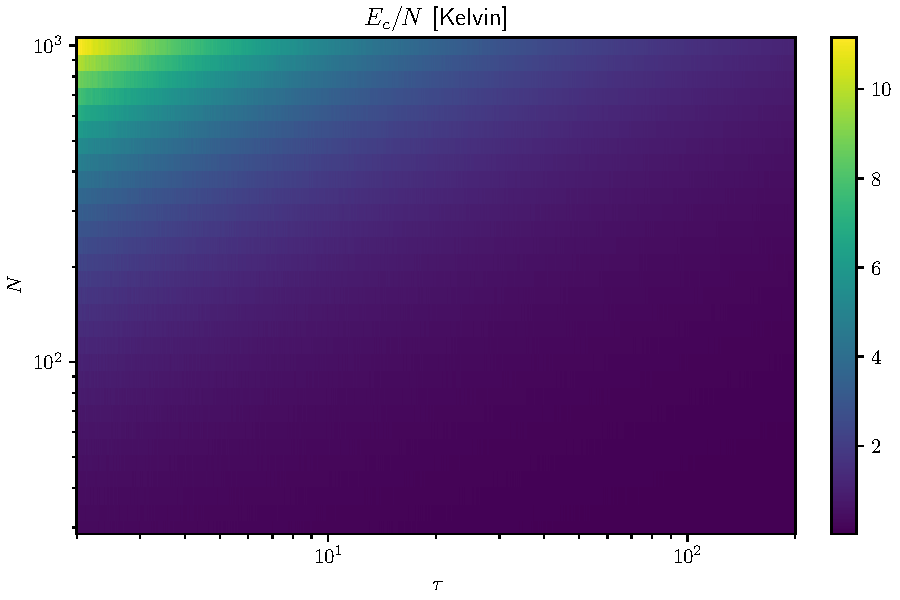
\includegraphics[width=\textwidth]{graphics/coulomb_energy_example@coulomb_energy.pdf}
	\end{center}
	\caption{Example dependence of $E_c/N$ to $N$ and $\tau$ for a trap of \ce{Yb^+} with secular frequencies of $(8.5, 8.5, 1.5) \mathrm{kHz}$, in the range of $\tau\in[2, 200]\mathrm{K}$.}\label{fig:coulomb_energy}
\end{figure}

To produce this color-mesh, we distributed the ions in space multiple times per $(\tau,N)$ point, until the relative standard deviation of all $E_c/N$ results in that point was lower then $0.12$ (arbitrary number), with a minimum of 5 distributions (also termed 'iterations'). Statistical results of figure~\ref{fig:coulomb_energy} is depicted in figures \ref{fig:coulomb_energy_std} and \ref{fig:coulomb_energy_iterations}.

Naturally, the value of the highest Coulomb energy found escalates with the trap's tightness, as can be seen in figure~\ref{fig:coulomb_energy_f_z}.

\begin{figure}
	\begin{center}
		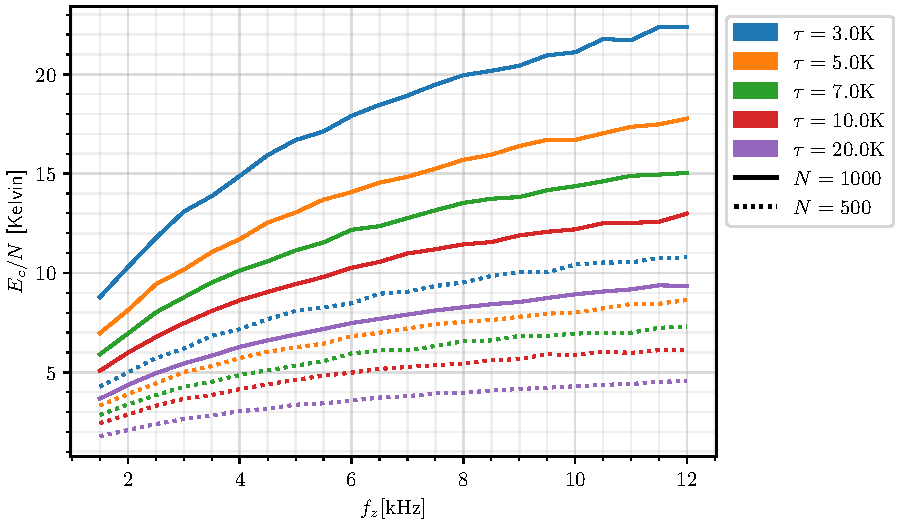
\includegraphics[width=\textwidth]{graphics/coulomb_energy_f_z.pdf}
	\end{center}
	\caption{The dependence of $E_c/N$ upon the z secular frequency, for a few specific $(\tau,N)$ pairs, and $f_x = f_y = 8.5\mathrm{kHz}$.}\label{fig:coulomb_energy_f_z}
\end{figure}

\subsubsection{Summary}

The Coulomb energy is not negligible for dense \& cold distributions. Our ability to initiate a distribution of ions in a thermodynamically stable set of positions is limited by the effects of strong Coulomb energy, and by the tightness of our trap. To avoid too strong Coulomb energy effects, we thereby avoid distributing ions in $T < 5\mathrm{K}$.\footnote{During the research period I tried to construct an algorithm that would get a real temperature $T \ne \tau$, $N$ and a set of secular frequencies, and compute a $\tau$ with which the system will be more thermodynamically stable initially. When this algorithm was used for a single ion species it was slightly effective. However when 2 ion species were used, (with different masses and different $\{k_i\}$ - see section~\ref{sec:theory/mathieu-inversly}), accommodating the algorithm for that case has proved to be too complex, and too slow.}

More importantly, we expect time dependent temperature measurements to be offset from the initial temperature $T_i$ on the order of magnitude of the Coulomb energy. Since we also wish to start cooling when the system is thermodynamically stable, the Coulomb energy offset requires us to wait for a few $\mathrm{ms}$, before beginning cooling, as can also be seen from the oscillations in figure. % TODO: \ref{fig:} from 

\subsection{A Non-Trivial Secular Frequency Mass Dependence}\label{ssec:non-trivial-mass-dep}

In my literature review I have seen no authors discuss the secular frequency related implications encountered when 2 different masses are trapped in the same Ion trap. This detail is particularly relevant to us, as we are interested in sympathetic cooling, and initiating our simulations in thermodynamic equilibrium, according to equation~\ref{eq:position-probability}.

Let's discuss this question in 1 spatial dimension: Given a $(a,q)$ pair producing a dimensionless secular frequency $\beta_0$ for mass $m_{cooler}$, what would be the secular frequency experienced by a mass $m_{target}$ experiencing the same forces? In a pure harmonic oscillator, the same $k = m_{cooler} \omega_{\mathrm{sec(cooler)}}^2 = m_{cooler} (\beta_0 \omega_\mathrm{rf}/2)^2$ is applied to any mass, and we get a secular frequency for $m_{target}$ of:

\begin{equation}
	\omega_\mathrm{sec(target)} = \omega_\mathrm{sec(cooler)}\sqrt{\frac{m_{cooler}}{m_{target}}} 
\end{equation}

Is that true in a Mathieu trap? The process of generating a dimensionless $(a,q)$ from the original equation of motion (equation \ref{eq:mathieu-source}) involves dividing the equation by the mass, meaning that $(a,q)\propto 1/m_{cooler}$. Hence the real secular frequency of $m_{target}$ can be obtained by calculating $\beta_{target}$ given the pair:

$$(a,q)\cdot \frac{m_{cooler}}{m_{target}}$$

The dependence of $\beta_{target}$ as a function of the mass ratio is depicted in figure~\ref{fig:mathieu-mass-dep}. This insight invites defining 2 decoupled, boolean parameters for the simulation, named \texttt{micromotion} \& \texttt{naive\_freqs}. Table~\ref{tbl:naive_freqs-micromotion} is a truth table explaining what trapping forces are applied in each combination of these parameters. A separate definition of these parameters is laid out afterwards for completeness.

\begin{figure}
	\begin{center}
		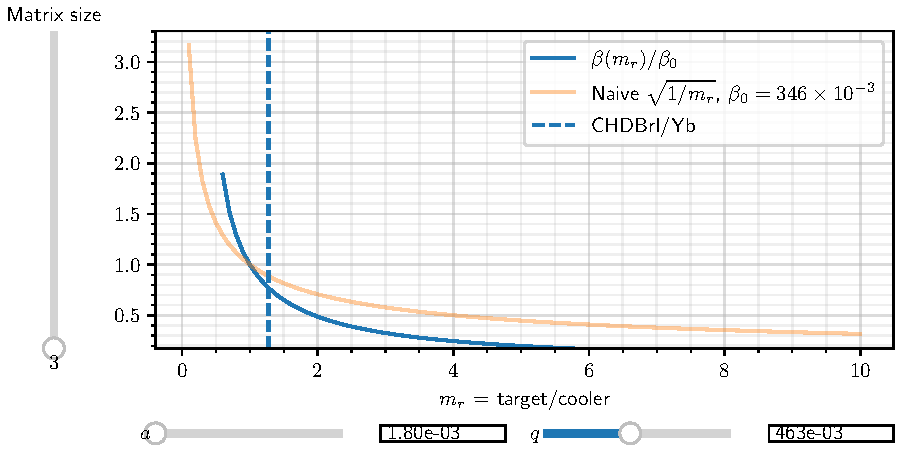
\includegraphics[width=\textwidth]{graphics/mathieu-mass-dep.pdf}
	\end{center}
	\caption{A Matplotlib interactive plot showing the non-trivial dependence of the secular frequencies of a 'target' mass (represented in blue), given a Mathieu trap with $(a,q)$ that define a certain secular frequency for a 'cooler' mass, termed $\beta_0$. The $(a,q)$ values used here, produce $\beta_0 = 2\cdot 8.5/50$ - like the $x$ \& $y$ axis Mathieu forces of figure~\ref{fig:LAMMPS_summarized_naive_freqs-micromotion}.}
	\label{fig:mathieu-mass-dep}
\end{figure}

\begin{table}[h]
\centering
\begin{tabularx}{\textwidth}{cccX}
\toprule
\texttt{mm} & $\sqrt{m_r}$ & \textbf{Physical} & \textbf{Description} \\
\midrule
$\checkmark$ & $\times$ & $\checkmark$ & A single electric field exhibiting 3 dimensional Mathieu equations - The only physically possible kind of trap, with non-trivial secular frequencies as presented in figure~\ref{fig:mathieu-mass-dep}. \\
\midrule
$\times$ & $\checkmark$ & $\times$ & A single \(k \mathbf{x}\)-like force is acting upon all ions — implementing the naive frequencies you'd expect from a perfect Harmonic oscillator. \\
\midrule
$\checkmark$ & $\checkmark$ & $\times$ & Two different Mathieu forces are applied to each mass, such that the naive frequencies related by $\sqrt{m_r} \equiv \sqrt{m_{cooler}/m_{target}}$ are experienced by the two ion species. \\
\midrule
$\times$ & $\times$ & $\times$ & Two different \(k \mathbf{x}\)-like forces are applied to each mass, such that the non-naive frequencies are experienced by the two ion species. \\
\bottomrule
\end{tabularx}
\caption{Truth table for \texttt{micromotion} (\texttt{mm}) and \texttt{naive\_freqs} ($\sqrt{m_r}$) combinations and their physical validity.}
\label{tbl:naive_freqs-micromotion}
\end{table}

\subsubsection*{\texttt{naive\_freqs} ($\sqrt{m_r}$)}

Controls whether the secular frequencies experienced by the target \ce{CHDBrI^+} ion are defined using the 'naive' $\sqrt{m_r}$ relation. Turning this option on naturally implements a trap that is not physically implementable.

\subsubsection*{\texttt{micromotion} (\texttt{mm})}

Controls whether the secular frequencies experienced by both ion species are implemented using a Mathieu like force like in equation \ref{eq:mathieu-source}, or using a perfect harmonic trap force like $k \mathbf{x}$. A perfectly harmonic trap is of course not implementable.

\subsubsection{LAMMPS Verification of Mathieu Understanding}

Now that we have gained confidence in our Mathieu solving capabilities, Let's demonstrate that indeed the reversely solved Mathieu equations presented in section~\ref{sec:theory/trapping} indeed produces $(a_i, q_i)$ pairs with the requested secular frequencies. Figure~\ref{fig:LAMMPS_summarized_naive_freqs-micromotion} demonstrates that decoupling the \texttt{micromotion} and \texttt{naive\_freqs} parameters was done successfully.

\begin{figure}
	\begin{center}
		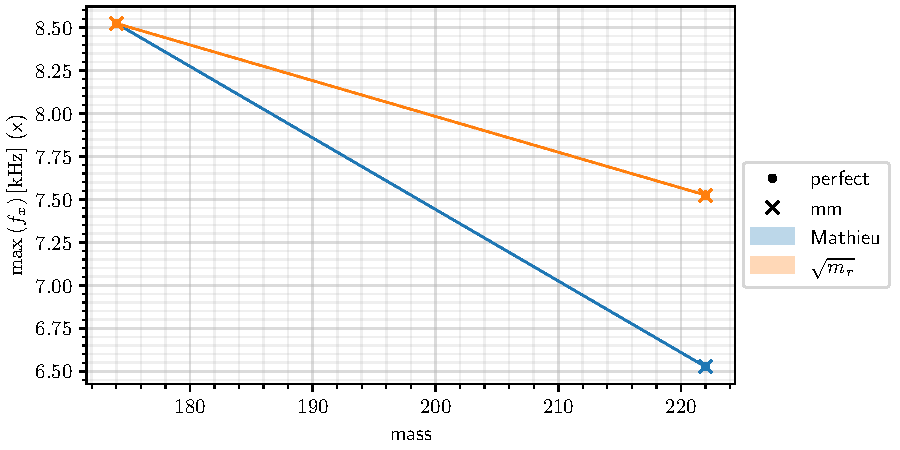
\includegraphics[width=\textwidth]{graphics/micromotion_and_sqrt_freqs_effect.pdf}
	\end{center}
	\caption{%
The collective $x$-axis movement's frequencies of a 2-species-mixed ion cloud, positioned in a spatial offset from the origin at $t=0$. Different markers represents whether \texttt{micromotion} was enabled, and the \texttt{naive\_freqs} parameter is represented in color. The frequencies were obtained via fitting\cite{scipy} the cloud's center to a cosine. Identical results can be obtained via using \texttt{numpy.fft.fft}\cite{numpy}.%
}
	\label{fig:LAMMPS_summarized_naive_freqs-micromotion}
\end{figure}

The color-varied behavior in figure~\ref{fig:LAMMPS_summarized_naive_freqs-micromotion}, demonstrates the non-negligible difference between the naive, $\sqrt{m_r}$-based calculation and the correct 'Mathieu frequencies' that are experienced in a real ion trap. The fact the two $\times$ \& $\circ$ markers appear on the same spots, proves that indeed the simulation code has successfully created the correct forces no matter whether \texttt{micromotion} was enabled or not. The only physically implementable dots are the blue $\times$ points.

\section{Cooling}

The theory of LASER cooling is well established for 2-level systems. The semi-classical model implemented in the simulations presented in this work is explained well in literature\cite{TannoudjiCooling,SteckCooling} and can be expressed as follows:

\begin{equation}
	\mathbf{F}(\mathbf{v}) = \frac{h \pi \gamma \hat{k}}{\lambda} \cdot \frac{\omega^2/2}{1/4 + \omega^2/2 + (d - \hat{k}\cdot\mathbf{v}/\lambda/\gamma)^2}
	\label{eq:laser-cool-force}
\end{equation}

Where:

\begin{itemize}
	\item $h$ is Planck's constant.
	\item $\hat{k}$ is the LASER's spatial direction.
	\item $\lambda$ is the cooling transition.
	\item $\gamma$, is the cooling transition's lifetime in Hz dimensions. The more commonly used $\mathrm{rad}/\mathrm{s}$ scaled lifetime is usually denoted as $\Gamma = 2\pi \gamma$.
	\item $d$ is the LASER's detuning normalized to $\Gamma$. Sometimes the not normalized detuning in the dimensions of $\mathrm{rad}/\mathrm{sec}$ is denoted as $\delta$ and with it we can denote $d \equiv \delta/\Gamma$.
	\item $\mathbf{v}$ is the velocity of the cooled atom.
	\item $\omega$ is the LASER's Rabi frequency normalized to $\Gamma/2\pi$. Very similarly to $d$ and $\delta$ the following can be stated: $\omega \equiv \Omega/\Gamma$.
\end{itemize}

% TODO: Explain also the more intuitive reason for putting an odd expression - the offset is apparent also without a Taylor expression - like in the seminar

In principal, there is a Taylor expansion for the above expression for low $\mathbf{v}/\lambda/\gamma$. Let's observe this expansion for a slightly simplified, 1 spatial dimensional form of the force - with $\mathbf{v} = (v,0,0)$ and $\hat{k} = (1,0,0)$:

\begin{equation}
	\frac{h \pi \gamma}{\lambda} \cdot \frac{\omega^2/2}{1/4 + \omega^2/2 + d^2} \left(
		1 + \frac{2d}{1/4 + \omega^2/2 + d^2} \cdot v/\lambda/\gamma
	\right)
	\label{eq:laser-cool-taylor-force}
\end{equation}

To understand the effect of the 0th order force component, let's observe a simplistic system of a 1 dimensional harmonic oscillator with a damping force of the form above:

\begin{equation}
	\ddot{x} = - \omega_{sec}^2 x + F_0/m - 2 \xi \omega_{sec} \dot{x}
\end{equation}

Where $\omega_{sec}$ is the secular frequency well defined by our trap as explained in section~\ref{sec:theory/trapping} and $\xi$ is derived from the 1st order force component in expression \ref{eq:laser-cool-taylor-force}. The well known solution is of the form: 

\begin{equation}
	x(t) = \frac{F_0}{m \omega_{sec}^2} + A e^{-\xi \omega_{sec} t} \sin(\sqrt{1-\xi^2}\ \omega_{sec} t + \phi)
\end{equation}

Where $A$ and $\phi$ are determined by initial conditions. The steady state's offset from the origin $F_0/m\omega_{sec}^2$ in the case of a LASER cooling force equals:

\begin{equation}
x_o = \frac{h \pi \gamma}{\lambda}\cdot\frac{\omega^2/2}{1/4+\omega^2/2 + d^2} \cdot\frac{1}{m \omega_{sec}^2}
\end{equation}

If we'll take:

\begin{itemize}
	\item Secular frequency $\omega_{sec}$ in the order of magnitude of $\sim 2\pi\cdot 1.5\mathrm{kHz}$.
	\item LASER intensity of $\omega \equiv \Omega/\Gamma = 1$.\footnote{See also relation to actual intensity in subsubsection \ref{sec:theory/cooling-summary}}
	\item A common LASER detuning of $d \equiv \delta/\Gamma = 1/2$. % TODO: Cite or footnote why is this considered common.
	\item \ce{Yb^+} and the cooling transition at $c/\lambda = 811.2891 \mathrm{THz}$ with the line width $\Gamma/2\pi \equiv \gamma = 19.6 \mathrm{MHz}$.\cite{RansfordThesis}
\end{itemize}

We'd get $x_o \approx 2.1 \mathrm{mm}$, where the trap's harmonic region is of about $25 \mathrm{mm}$ from the origin. This offset might not be very significant for only LASER cooling a single ion like \ce{Yb^+}, but sympathetic cooling will suffer from this offset, as the target molecule won't experience an identical offsetting force, and would not collide frequently enough with the cooling ion and therefor will not lose kinetic energy, as seen in figure~\ref{fig:LASER-cool-offset3D}. Naturally increasing the secular frequencies of the trap greatly reduces this offset, but our trap's design doesn't allow much higher secular frequencies.

\begin{figure}
    \centering
    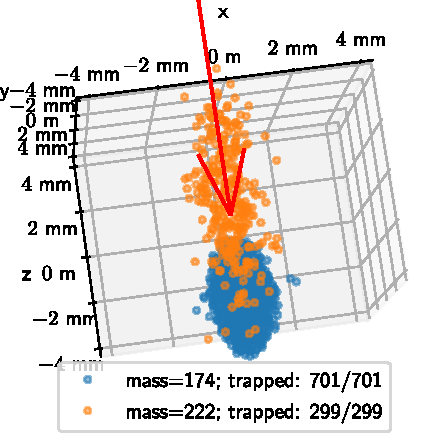
\includegraphics[width=0.5\textwidth]{graphics/LASER-cool-offset3D.pdf}
	\caption{The offset produced by a single LASER coming in the $z$ axis, where secular frequencies are $f_x = f_y = 8.5\ \mathrm{kHz}$ and $f_z = 1.5\ \mathrm{kHz}$. The offset measured fits exactly the analytical prediction of $x_0 \approx 2.1 \mathrm{mm}$.}
	\label{fig:LASER-cool-offset3D}
\end{figure}

% TODO: Consider citing and discuss a bit about what kind of forces other people use in simulations - discuss with Yuval about the fact the real expression for any \hat{k} and \mathbf{v} includes many cross-terms and looks very messy.

% TODO: Ask Yuval whether more references for using counter-propagating beams would be useful here:
As suggested in a more classical LASER cooling model presented by Dan Steck\cite{SteckClassicalCooling}, we can use 2 counter propagating LASER beams, that will apply 2 forces which sum up to $\mathbf{F}(\mathbf{v}) - \mathbf{F}(-\mathbf{v})$, forming an odd function in $\mathbf{v}$, with no 0th order component. Creating 2 such counter-propagating beams in experiment is simply done with a mirror. However, the vacuum chamber's windows induce a small attenuation on the intensity, as illustrated in figure~\ref{fig:windows-attenuation}.

\begin{figure}[h!]
	\begin{center}
		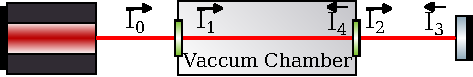
\includegraphics[width=0.95\textwidth]{graphics/windows-attenuation.pdf}
	\end{center}
	\caption{The effect of the Vaccum Chamber's windows' attenuation upon the LASER cooling intensities.}\label{fig:windows-attenuation}
\end{figure}

Since $\omega \equiv \Omega/\Gamma$ and $I \propto \Omega^2$, if we'd define\footnote{The experimentalist's most intuitive measurement is to measure $I_2/I_0$, but it should equal $I_4/I_1$ assuming all windows are made of identical glass, and the intensity lost in the mirror is 0.} $\alpha \equiv I_4/I_1$, the actual force we are imposed to apply upon our ions is:

\begin{equation}
	\mathbf{F}(\mathbf{v}, \omega) - \mathbf{F}(-\mathbf{v}, \sqrt{\alpha}\omega)
\end{equation}

Causing a slight imperfect oddness (with respect to $\mathbf{v}$) of the force, depending on the windows attenuation parameter $\alpha$.

\subsection{Expected Behavior of Detuning \& Intensity parameters}

% TODO: Think about this content... Do I really want it?

Without simulating, it is interesting to wonder: What would be the ideal detuning ($\delta$) and intensity ($\Omega$) given an ion cloud in temperature $T$? This depends upon the dependence of the effectiveness of the LASER cooling force. As for the detuning, the intuitive answer would be:

\begin{equation}
	d_\mathrm{opt} = \frac{\sqrt{K_\text{B} T/m}}{\lambda\gamma}
	\label{eq:back-of-envelope-detuning-T}
\end{equation}

Such that the most common velocity $v = \sqrt{K_\text{B} T/m}$, along with this detuning, is minimizing the denominator of force expression \ref{eq:laser-cool-force}. As for the optimal intensity, there is no clear answer that the force expression yields. A generalized way to answer the question laid out here is to ask:

Given a Maxwell-Boltzmann distribution of velocities, for which $d$ and $\omega$ is the overlap integral \ref{eq:laser-cool-overlap-integral} maximized?

\begin{equation}
	\int_{-\infty}^\infty\,\mathrm{d}v\exp\left(-\frac{m v^2}{2 K_\text{B} T}\right) \sum_\pm \frac{\pm\omega^2}{1/4 + \omega^2/4 + (d \mp v\lambda\gamma)^2}
	\label{eq:laser-cool-overlap-integral}
\end{equation}

Where the $\pm$ summation is implementing the counter propagating beams force summation. Figure~\ref{fig:laser-cool-optimal-overlap} presents the results of the maximisation for a wide range of temperatures. The resemblance of the intuitive 'back of the envelope' guess of expression \ref{eq:back-of-envelope-detuning-T} to the overlap-integral based solution is satisfactory.

\begin{figure}
	\begin{center}
		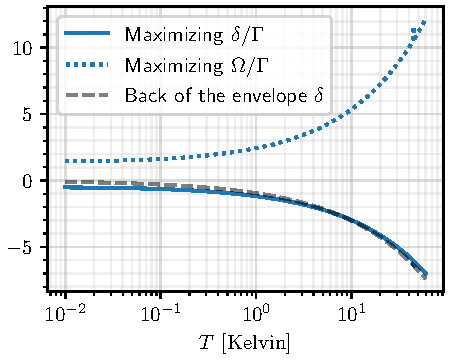
\includegraphics[width=0.5\textwidth]{graphics/laser_cool_overlap.pdf}
	\end{center}
	\caption{Optimal LASER cooling parameters calculated for a general ion cloud, using a maximisation of integral \ref{eq:laser-cool-overlap-integral}. The 'Back of the envelope' line is of \ref{eq:back-of-envelope-detuning-T}. The maximisation was done using \texttt{scipy.optimize.minimize} with \texttt{method='TNC'}\cite{scipy}. Similar results were obtained with other optimization methods, but this was the fastest method that also produced smooth results.}
	\label{fig:laser-cool-optimal-overlap}
\end{figure}

This result can be used to optimize the cooling process via changing the detuning \& intensity of the cooling LASERs dynamically. Writing an algorithm that would play with the detuning \& intensity to optimize the cooling according to intermediate temperature measurements could be an interesting topic for further research, either via simulations or directly in experiment.

\subsection{Summary}\label{sec:theory/cooling-summary}

This is a good place to pause and list all the simulation parameters we collected from the theory above:

\begin{itemize}
	\item The LASER cooled ion. Choosing an ion and a cooling transition is effectively choosing $\lambda$, $\gamma$ and the mass $m$.\footnote{Cooling transitions and line-widths were taken from \cite{CoolingBeParameters,CoolingCaParameters1,CoolingCaParameters2,RansfordThesis,RadiumData}}. Current experimental efforts as well as all simulations presented focus on \ce{Yb^+}, but in principal this parameter is not hard-coded, and 
	\item The normalized LASER's intensity $\omega \equiv \Omega/\Gamma$.
	\item The normalized LASER's detuning $d \equiv \delta/\Gamma$.
	\item The spatial direction(s) of the LASER(s). This can be parameterized by a list of $(\theta, \phi)$ pairs - a pair per LASER, defining each LASER's $\hat{k}$ using a spherical coordinates transformation.
	% TODO: Consider whether adding this
	%\item Whether to use the approximated Taylor expression with only the 1st order term. This is not really a physical simulation parameter, but it was studied because I couldn't find simulations simulations in literature not using the approximation.
	\item The Vacuum chamber's windows' attenuation. Our experiment's attenuation is $\alpha = 0.7$, and most simulations use this value.\footnote{Besides figure ... which displays it's effect.}
	% TODO: \ref{fig:windows-attenuation-effect} in the results
\end{itemize}

Lastly, the relation of the Rabi frequency $\Omega$ to the actual LASER intensity\cite{CJFootOmega2I}, is worth mentioning\footnote{The software is capable of displaying $\Omega$ dependence in the scale of the intensity $I$, but this behavior wasn't activated in the results presented.}:
% TODO: Make sure the above footnote is correct

\begin{equation}
	I = \frac{2\pi h c \Gamma}{3 \lambda^3} \cdot \left(\frac{\Omega}{\Gamma}\right)^2
	\label{eq:omega2intensity}
\end{equation}

\section{Technical Parameters}

\subsection{Time Periods}

% TODO: This should be rephrased

To fully define a simulation, one has to define a few more parameters. Two of which are related to the timeline and are called \emph{cooling} and \emph{stabilizing} time. The cooling time period has trivial meaning and increasing it can be usually interesting but naturally the price is higher computing resources demands. The stabilization time is the time since $t=0$ up to the point where the LASER cooling force enters.

For researching cooling parameters, and for most initial temperatures, there is no need for more then $5-7\mathrm{ms}$ of stabilizing time, just to let the thermodynamic instabilities of the initial conditions minimize. Figure~\ref{fig:T-stabilizes-example} can serve as a good example in which the width of $T(t)$ before the LASER cooling starts, decreases enough after $6 \mathrm{ms}$, which is good enough for several initial temperatures.

\begin{figure}
	\centering
	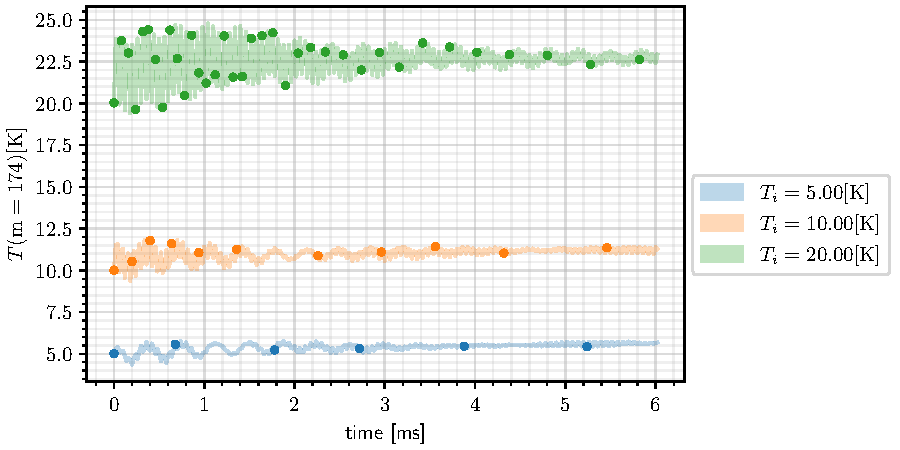
\includegraphics[width=\textwidth]{graphics/T-stabilizes-example.pdf}
	\caption{Several temperature measurements of \ce{Yb^+}, without LASER cooling, and $6\ \mathrm{ms}$ stabilization time. RF heating is observed for $T_\mathrm{initial} = 5\ \mathrm{ms}$.}
	\label{fig:T-stabilizes-example}
\end{figure}

Another usage for varying the stabilization time, is for measuring the eigenfrequencies of the trap, without cooling ($0$ cooling time), and all cooling parameters irrelevant.

\subsection{Time Dividing Fineness}

Another fairly technical parameter is the fineness of the time division. As further justified in section~\ref{ssec:T_rf_type}, we want to always divide the simulation to an integer number of RF cycles. Since the RF frequency is also the highest frequency of the system, the natural thing to do is to divide each RF cycle to an integer number of steps, and this slightly arbitrary parameter is called the RF divisor. There is no theory that predicts an optimal RF divisor, and still this is an important technical detail.

One can perform many simulations with a certain RF divisor, and only in a specific simulation, in a specific advanced time, notice a certain ion has experienced a non-physically strong Coulomb force, causing it to fly way very far away, making the temperatures measurements noisy throughout the rest of the simulation, and hence essentially incorrect. With way too low RF divisors the temperatures measurements will be noisy and incorrect from the start. After a few months of optimizing this parameter, a value for the RF divisor was stabilized around $\approx 1500$, depending on the trap's RF frequency. See figure~\ref{fig:convergence-example}.

\begin{figure}
    \centering
	\begin{subfigure}{0.59\textwidth}
    	\centering
    	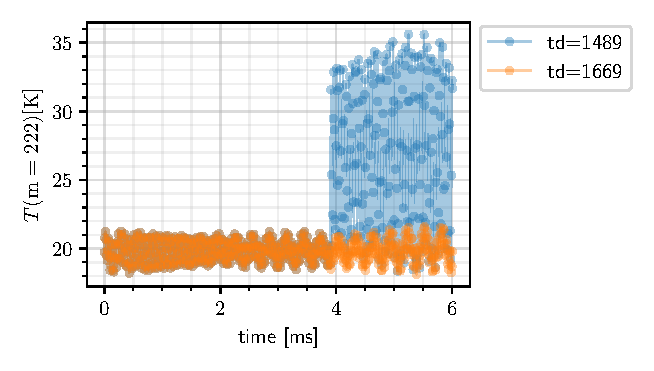
\includegraphics[width=\linewidth]{graphics/convergence-example.pdf}
		\caption{The temperatures measurement reflects there are ions which are too hot, and increasing the RF divisor parameter \texttt{td} fixes this issue.}
	\end{subfigure}
	~
	\begin{subfigure}{0.38\textwidth}
    	\centering
    	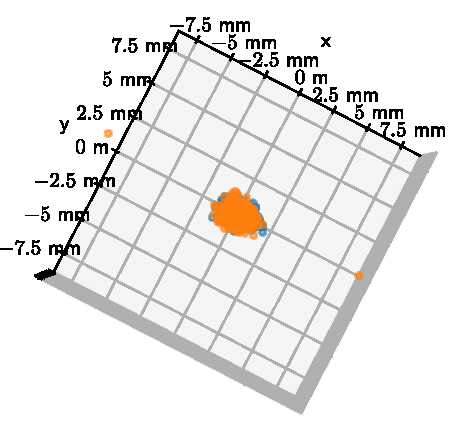
\includegraphics[width=\linewidth]{graphics/coulomb-explosion.pdf}
		\caption{The coulomb force made 2 \ce{CHDBrI^+} ions fly roughly $8\ \mathrm{mm}$ from the center.}
	\end{subfigure}
	\caption{\emph{Coulomb explosion}, demonstrated both in 3D simulation and in $T(t)$ measurement.}
	\label{fig:convergence-example}
\end{figure}

To further tighten the demand of the RF division's independence from potential numerical errors, a prime number was chosen\cite{primesieve}.

\subsection{Initial Conditions}

Lastly, the initial conditions were obtained using a random number generator with a specific seed. Each seed integer represents a reproducible set of initial conditions, given the algorithm distributing positions and velocities stays the same. To decouple the (small) effects of initial conditions upon the results, the same simulations but with different seeds were ran, and in most results displayed this dimension was averaged over.

\section{Measuring}\label{sec:intro/-y-options}

Naturally, the main result that interests us is the temperature. Which is essentially a common measure for the average kinetic energy, and in our case, since we use a VMI, it is a measure of the velocities' distribution's width. A physically related property of our ion clouds is the size, that can be measured per axis simply via a \texttt{std}. As for the temperatures, there are a few more ways to measure them, laid out below. 

\subsection{Temperature's Random Variables}

Under the approximated treatment of the Ion trap's potential as a perfect harmonic potential, and with the long range Coulomb potential neglected, one can treat the positions analogously, and hence almost identically to the velocities. This is done by multiplying each particle's position $x_i$ in the $i$'th axis, by $2\pi f_i x_i$, where $f_i$ is the secular frequency of the Ion trap in the $i$'th axis.\footnote{Although not implied by an existence of an additional index besides $i$, there is a different, non-trivial set of $f_i$ secular frequencies per particle species, as described in section~\ref{ssec:non-trivial-mass-dep}.}

% TODO: Use labels per these temperatures related subsections, and \ref to them in the technical part of the thesis.
\subsection{Temperature's Probabilistic Methods}\label{ssec:T_method}

Given $N$ particles, which were 'measured' during the computer simulation in a certain time, 2 arrays of shapes \texttt{(N,3)} are obtained for velocities and positions. The positions' array can be scaled by the proper secular frequencies as described above, and the question of how to compute a temperature given such an array has multiple legitimate answers. To layout all available answers we'll denote the random variable $u_i \in \{v_i, 2\pi f_i x_i\}$ for axis $i$. The $i$'th slice of length \texttt{N} from the above \texttt{(N,3)} shaped array is a distribution of the $u_i$ random variable.

One simple answer which is most intuitive in the context of VMI based measurements is to simply compute $m \mathrm{Var}(u_i)/K_\text{B}$, as derived from the Maxwell-Boltzmann distribution expression:

\begin{equation}
	f(\mathbf{u}) \mathrm{d}^{3}\mathbf{u} = \left[\frac{m}{2\pi k_{\text{B}}T}\right]^{3/2}\,\exp \left(-{\frac {m \mathbf{u}^2}{2K_\text{B} T}}\right) \mathrm{d}^{3}\mathbf{u}
\end{equation}

Another approach, is to integrate over a solid angle of $\mathbf{u}$ in the probabilistic model above, and write a speeds-like distribution function:

\begin{equation}
	f(|\mathbf{u}|) = \left[{\frac{m}{2\pi K_\text{B} T}}\right]^{3/2} 4\pi |\mathbf{u}|^{2}\exp\left(-{\frac{m |\mathbf{u}|^{2}}{2k_{\text{B}}T}}\right)
\end{equation}

Which has a variance equal to $K_\text{B} T/m \cdot (3 - 8/\pi)$, and a squared mean equal to $K_\text{B} T/m \cdot 8/\pi$, thus providing 2 more methods to calculate a temperature given a \texttt{(N,3)} shaped array of either positions or velocities.

\subsection{Temperature Under the Secular Approximation}\label{ssec:T_rf_type}

In addition to the velocities and/or positions choice of random variable(s), and in addition to the above probabilistic model approaches, one has to decide how to imitate the secular approximation computationally. The physical justification for doing it, is the fact that in a crystal phase (which we aim achieving), the movement of the ions is strongly coupled to the RF field which we have direct control over. Essentially the model states that the collective movement due to the RF field is predictable and so well defined, that it is not a random variable.

Experimentally speaking, we are capable of measuring positions and velocities always at the beginning/end of each RF cycle, and hence always use an integer number of RF cycles. This is the simplest and probably the only way of implementing a secular approximation experimentally, and it should work best for ions that have formed a crystal. In the following, we'll describe what other techniques are available to a computer simulation that might help achieve time dependent, secularly approximated temperature measurements.\footnote{There's also a technical motivation to imitate some kind of secular approximation when measuring temperatures, and that is reducing the amount of disk writes required when simulating $\sim 3,000$ RF cycles divided to $\sim 1500$ time steps. Reducing the amount of disk writes not only reduces disk usage of simulation result files, but also speeds up the total time required for simulating.}

% TODO: Cite stuff from zothero regarding RF averaging..
Besides sampling the velocities and positions in the beginning of each RF cycle, many simulations based research found in literature average over an RF period each particle's per-axis velocity, and then construct a temperature. You might hope that the same can be done for $2\pi f_i x_i$, but apparently, even for ion clouds initiated in a thermal gas phase equilibrium in temperatures as low as $5\mathrm{K}$, each particle reaches many spatial areas of the trap, and it's RF averaged position produce (incorrect) temperatures in the $\mathrm{\mu K}$ regime! This proves that this approach is not accurate also for the velocities, at least for gas like phases, as it suggests that ions go through a big part of the phase-space. Never the less, I decided to do save the RF averaged velocities (but not the positions) to the disk during simulations, and the software displaying the simulation results provides the option to use this data.

Another interesting RF cycles related option, is to sample the velocities and positions in the middle of each RF cycle - where the kinetic energy induces by the RF field should be at it's peak. The difference from the energies in the beginning of the RF cycles may help extract the RF motion energy. This data was also saved for both positions and velocities, for consistency.

\subsection{Temperatures Options Summary}\label{ssec:T-options-summery}

The above temperatures related options are modeled in software as 3 dimensions with the names and symbolic optional values as defined in table~\ref{tbl:T_methods}. We can select specific, multiple temperature values and average over the different methods, coordinates and RF handling methods. A common example is to take the positions and velocities sampled in the beginning of each RF cycle ($\mathrm{min}\left(\circlearrowright\right)$), and calculate the temperature according to all \texttt{T\_method}s. Whatever specific \texttt{T\_coord}s / \texttt{T\_rf\_type}s / \texttt{T\_method}s were chosen, the code analyzing and displaying the simulation results averages over these dimensions for each time index separately.\footnote{Technically, the temperatures obtained from the RF averaged ($\left\langle\circlearrowright\right\rangle$) positions ($\overrightarrow{\omega x}$) are considered \texttt{NaN} and hence ignored.}

\begin{table}
\begin{tabular}{l||l|l|l|l|l}
Dimension   & \multicolumn{5}{c}{Optional values}\\
\hline\hline
% TODO: Maybe T_coord is not a good name?
 \texttt{T\_coord}   & $\vec{v}$                                    & \multicolumn{2}{l}{$\overrightarrow{\omega x}$} \\
\hline
\texttt{T\_rf\_type} & $\left\langle\circlearrowright\right\rangle$ & $\mathrm{min}\left(\circlearrowright\right)$ & \multicolumn{2}{l}{$\mathrm{max}\left(\circlearrowright\right)$} \\
\hline
\texttt{T\_method}  & $\mathrm{Ave}\left(|u|\right)^2(\pi/8)$      & $\mathrm{Var}\left(|u|\right)/(3 - 8/\pi)$   & $\mathrm{Var}\left(u_x\right)$               & $\mathrm{Var}\left(u_y\right)$ & $\mathrm{Var}\left(u_z\right)$ \\
\hline
\end{tabular}
\caption{Ways to measure temperatures, obtained from a generalized maxwell-Boltzmann model. $\circlearrowright$ marks an RF cycle, and $\left\langle\circlearrowright\right\rangle$ marks an average over RF cycle. The functions $\mathrm{Ave}$ and $\mathrm{Var}$ operate upon a 1 dimensional array of length $N$ - the number of per specie's particles.}
\label{tbl:T_methods}
\end{table}

\subsection{Further Summarizing Analyzes}\label{ssec:intro/SummarizedMeasurement}

Up until now we discussed time dependent properties of our ion clouds - the per spatial axis size and the various temperatures. We can also summarize these results to obtain various measures of how fast did we cool our ions, and how much smaller did the cloud get due to the LASER cooling etc. This is termed both in the code and here as summarized results.

The simplest summarized result type is the temperature/size after the cooling process, which is defined (slightly arbitrarily) as the average temperature/size of the ion cloud in the last 1/4 of the time before cooling or before the end. The first \textit{part} is referred to as \textit{stabilizing part} and the later \textit{cooling part}. The standard deviation of the temperature/size in each such \textit{part} defines the uncertainty for each such summarized measurement. The size measurement, both in the time dependent form and in the summarized form depends on the spatial axis (x,y,z), and the temperatures, in either the summarized or time dependent form, depend on the 3 dimensions described in section~\ref{ssec:T-options-summery}.

Another summarized measurement is the cooling frequency, defined (for simplicity, only for temperatures) as follows: Given a $T(t)$ defined using any of the parameters of section~\ref{ssec:T-options-summery}, we take $\mathrm{Log}(T(t)/\mathrm{kelvin})$, and apply a continuous piecewise linear fit\cite{pwlf}, with 2 segments. This gives 2 cooling frequencies in the units of $\mathrm{kHz}$ that depend on a dimension referred to as \texttt{regime} - corresponding to the segments. This design choice stems from the observation that in many simulations most of the ion cloud is cooled quickly and efficiently whereas afterwards the rest of the cooling happens in a mixed thermodynamic phase of an ion crystal (massive and highly charged) with a gas of ions surrounding it. The initial, faster and more efficient part of the cooling process corresponds to the 1st segment of exponential temperature decay, and the rest of the cooling is significantly slower, and hence invite defining a 2nd segment of cooling.

Lastly, only for verifying the frequencies expected from the Mathieu equations of the ion trap, as explained in section~\ref{sec:theory/trapping}, we define the following analysis referred to as the \textit{cloud's frequencies}: Given the time dependent positions of all ions, we average over the ions to get the cloud's center position (still time and spatial axis dependent). With it, we can take the Fourier transform and get the dominant frequency via \texttt{scipy.signal.find\_peaks}\cite{scipy}, or simply via \texttt{numpy.argmax}\cite{numpy}. If the collective movement is very harmonic (due to e.g collective offset in which the ion cloud was intentionally placed at $t=0$), a fit for a $\cos(2\pi f x_i + \phi)$ can be attempted, and the fit's frequency is the dominant frequency of movement. The time range of the simulation dictates the uncertainty in the dominant frequency obtained via a Fourier transform, and the dominant frequency of the fit produces uncertainties via the covariance matrix returned by \texttt{scipy.optimize.curve\_fit}.

